\chapter{Apprentissage des modèles et résultats}

\section{Introduction}

La réalisation d'une application basée sur l'exploitation des méthodes de
l'apprentissage automatique est effectuée en deux étapes : la première est
la conception d'un modèle capable d'apprendre à faire le traitement demandé, et
la deuxième est l'exécution de l'apprentissage de ce modèle en utilisant
les données disponibles.

La première étape était le sujet du chapitre précédent, où nous avons conçu nos
architectures de réseaux de neurones convolutionnels et nous avons établi les
structures comportant nos données. La deuxième étape, qui est le sujet de ce chapitre,
consiste à fournir les données aux réseaux répétitivement afin de leur permettre
de trouver la fonction générale du problème adressé qui projette chaque donnée
entrante vers la classe de la sortie correspondante.

Nous commençons par la description de nos données et leurs formats, suivie de
la présentation des outils matériels et logiciels utilisés dans ce projet, et puis
nous analysons les résultats obtenus de l'apprentissage automatique et nous
finissons par la mise en œuvre du modèle dans une application développée
afin de permettre à un utilisateur de trouver la classe de distances à partir d'une
image.

\section{Les données utilisées}

\subsection{Les sources}

Nous avons collecté nos données à partir de deux endroits différents afin de
construire deux ensembles de données, dont chacun contient des centaines d'images
et leurs distances. Le plus petit ensemble d'images a été
pris dans les salles du \keyword{centre culturel universitaire (CCU) des sciences techniques},
et l'autre ensemble a été pris dans les locaux du \keyword{département d'informatique} de
notre université.

L'ensemble des données du CCU contient 985 instances, dont 788 sont
utilisées pour effectuer l'apprentissage, les instances restantes étant réservées
comme données pour effectuer la validation des performances du modèle.
Par ailleurs, l'ensemble de données du département d'informatique contient 3068
instances, dont 2454 sont utilisées pour l'apprentissage et les restantes pour
la validation.

Les images de l'ensemble de données du CCU représentent des scènes d'intérieur
contenant des meubles comme les chaises et les tables en plus des murs.
Les niveaux de luminosité dans les scènes sont différents car certaines sont plus
éclairées que d'autres à cause de l'utilisation de la lumière artificielle (les
lampes des salles ou le feu du robot). La plupart des distances figurant dans
cet ensemble sont petites. De ce fait, les données sont très biaisées.

\bigskip

\begin{figure}[h]
\centering
\begin{subfigure}{0.125\textwidth}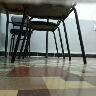
\includegraphics[width=\textwidth]{CCU1}\end{subfigure}
\begin{subfigure}{0.125\textwidth}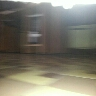
\includegraphics[width=\textwidth]{CCU2}\end{subfigure}
\begin{subfigure}{0.125\textwidth}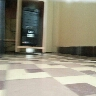
\includegraphics[width=\textwidth]{CCU3}\end{subfigure}
\begin{subfigure}{0.125\textwidth}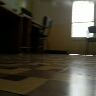
\includegraphics[width=\textwidth]{CCU4}\end{subfigure}
\begin{subfigure}{0.125\textwidth}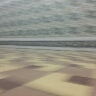
\includegraphics[width=\textwidth]{CCU5}\end{subfigure}
\begin{subfigure}{0.125\textwidth}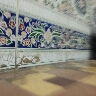
\includegraphics[width=\textwidth]{CCU6}\end{subfigure}
\begin{subfigure}{0.125\textwidth}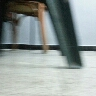
\includegraphics[width=\textwidth]{CCU7}\end{subfigure}
\begin{subfigure}{0.125\textwidth}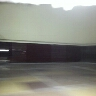
\includegraphics[width=\textwidth]{CCU8}\end{subfigure}
\begin{subfigure}{0.125\textwidth}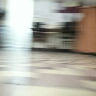
\includegraphics[width=\textwidth]{CCU9}\end{subfigure}
\begin{subfigure}{0.125\textwidth}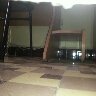
\includegraphics[width=\textwidth]{CCU10}\end{subfigure}
\begin{subfigure}{0.125\textwidth}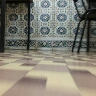
\includegraphics[width=\textwidth]{CCU11}\end{subfigure}
\begin{subfigure}{0.125\textwidth}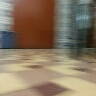
\includegraphics[width=\textwidth]{CCU12}\end{subfigure}
\begin{subfigure}{0.125\textwidth}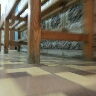
\includegraphics[width=\textwidth]{CCU13}\end{subfigure}
\begin{subfigure}{0.125\textwidth}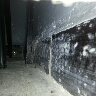
\includegraphics[width=\textwidth]{CCU14}\end{subfigure}
\caption{Des images de l'ensemble de données du CCU}
\end{figure}

Les images de l'ensemble de données du département sont généralement des scènes
d'extérieur constituées de sols, de plantes, de murs et de portes de couleurs uniformes.
La variance de la luminosité n'est pas forte vu que la source de la lumière dans
la majorité des images est le soleil. Le problème du biaisement des données est
moins effectif dans cet ensemble bien qu'il y ait peu de grandes distances par rapport
au reste.

\bigskip

\begin{figure}[h]
\centering
\begin{subfigure}{0.125\textwidth}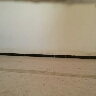
\includegraphics[width=\textwidth]{Info1}\end{subfigure}
\begin{subfigure}{0.125\textwidth}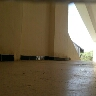
\includegraphics[width=\textwidth]{Info2}\end{subfigure}
\begin{subfigure}{0.125\textwidth}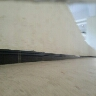
\includegraphics[width=\textwidth]{Info3}\end{subfigure}
\begin{subfigure}{0.125\textwidth}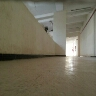
\includegraphics[width=\textwidth]{Info4}\end{subfigure}
\begin{subfigure}{0.125\textwidth}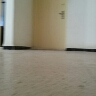
\includegraphics[width=\textwidth]{Info5}\end{subfigure}
\begin{subfigure}{0.125\textwidth}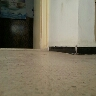
\includegraphics[width=\textwidth]{Info6}\end{subfigure}
\begin{subfigure}{0.125\textwidth}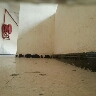
\includegraphics[width=\textwidth]{Info7}\end{subfigure}
\begin{subfigure}{0.125\textwidth}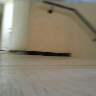
\includegraphics[width=\textwidth]{Info8}\end{subfigure}
\begin{subfigure}{0.125\textwidth}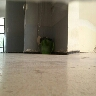
\includegraphics[width=\textwidth]{Info9}\end{subfigure}
\begin{subfigure}{0.125\textwidth}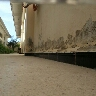
\includegraphics[width=\textwidth]{Info10}\end{subfigure}
\begin{subfigure}{0.125\textwidth}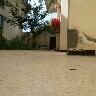
\includegraphics[width=\textwidth]{Info11}\end{subfigure}
\begin{subfigure}{0.125\textwidth}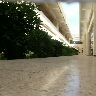
\includegraphics[width=\textwidth]{Info12}\end{subfigure}
\begin{subfigure}{0.125\textwidth}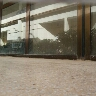
\includegraphics[width=\textwidth]{Info13}\end{subfigure}
\begin{subfigure}{0.125\textwidth}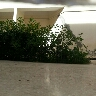
\includegraphics[width=\textwidth]{Info14}\end{subfigure}
\caption{Des images de l'ensemble de données du département d'informatique}
\end{figure}

\subsection{Le format et l'organisation}\label{subsec:format}

Les données se composent de deux types : des données pour l'entrée du modèle
qui sont les images capturées par la camera, et des données pour la sortie
qui sont les distances respectives mesurées par les capteurs ultrasoniques.

Chaque image est sauvegardée comme un fichier binaire sous le format JPEG~\cite{wallace1992jpeg}
(ayant l'extension \texttt{jpg}). Les images sont nommées par la composition du
préfixe \texttt{IMG\_} et un identificateur unique représentant le temps de la
prise. Elles sont toutes groupées dans un seul répertoire.

\parbox[][2em][]{\textwidth}{}

\begin{figure}[h]
  \centering
  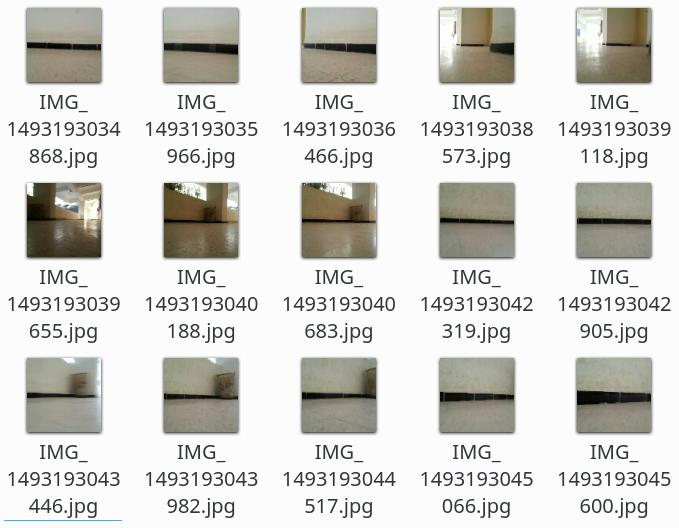
\includegraphics[width=0.75\textwidth]{Info-images}
  \caption{Des fichiers d'images successifs de l'ensemble de données du département}
\end{figure}

\parbox[][1.5em][]{\textwidth}{}

Les distances sont sauvegardées dans un fichier sous format CSV (comma-separated
values)~\cite{shafranovich2005common}, qui est un format textuel ayant comme rôle de représenter
les données tabulaires. Les lignes de ce fichier correspondent aux lignes du tableau
et les valeurs entre les séparateurs des colonnes aux données du tableau.
Le nombre de lignes dans ce fichier est égal au nombre d'images dans le
même répertoire car chaque ligne correspond à une image.

Le fichier qui contient les distances a le nom de \texttt{Distances.txt} et est
structuré en quatre colonnes séparées par le caractère \fbox{\texttt{,}}. La première
colonne contient les identificateurs des images, et les colonnes suivantes
représentes les distances mesurées pour chaque image.

\lstinputlisting[firstline=723,lastline=734,float=h,firstnumber=723,
caption=La partie du fichier des distances correspondante aux fichiers précédents]
{../Data/Info/train/Distances.txt}

L'ensemble des images et du fichier de distances sont éclatés en deux sous-ensembles
de tailles différentes. Le plus grand sera utilisé pour effectuer l'apprentissage,
et le plus petit sera réservé pour la validation. La structure de chaque
sous-ensemble est identique à celle de l'ensemble d'origine.

\section{Les technologies utilisées}

L'un des problèmes majeurs dans l'apprentissage automatique avec les réseaux
de neurones est leur consommation importante de temps d'exécution et d'espace
en mémoire centrale au moment de l'apprentissage.

Afin de minimiser l'effet de ce problème, nous avons besoin de deux choses.

\begin{itemize}
  \item Un matériel puissant permettra de disposer plusieurs unités de calcul
  pour le calcul parallèle, et possédant un espace considérable en mémoire
  centrale. Il permettra aussi, en mémoire secondaire, de stocker et charger les
  données de l'apprentissage ainsi que les paramètres trouvés et les performances
  sauvegardées au moment de l'apprentissage.
  \item Il faut aussi réaliser un programme optimal en termes de complexité et efficace du
  point de vue de l'exploitation des ressources matérielles.
\end{itemize}

\subsection{Le matériel}

Nous avons choisi d'exécuter notre programme d'apprentissage sur des machines de
\keyword{Google Cloud Platform}. Cette plateforme offre plusieurs services de calcul, de stockage,
de développement et de déploiement des applications basées sur les technologies
de \keyword{l'informatique en nuages} (cloud computing). Cette plateforme nous convient spécialement vu la facilité
de son utilisation et la qualité de ses services. De plus, elle offre un grand crédit
comme bonus initial pour les nouveaux utilisateurs, ce qui nous a permis de profiter de toutes ses
fonctionnalités gratuitement dans ce projet.

\begin{figure}[h]
  \centering
  
\includegraphics[width=0.5\textwidth]{gcp-logo}
  \caption[Le logo officiel du Google Cloud Platform]{Le logo officiel du Google Cloud Platform~\cite{gcp}}
\end{figure}

Le service qui nous intéresse est \keyword{Compute Engine}. Il nous permet de
créer une machine virtuelle ayant les caractéristiques matérielles pour notre tâche.
Les plus importantes sont le nombre des unités de traitement
centrales virtuelles (vCPU) et leur fréquence, la taille de la mémoire centrale
(RAM), et l'espace du stockage permanent dans le disque dur.

\begin{figure}[h]
  \centering
  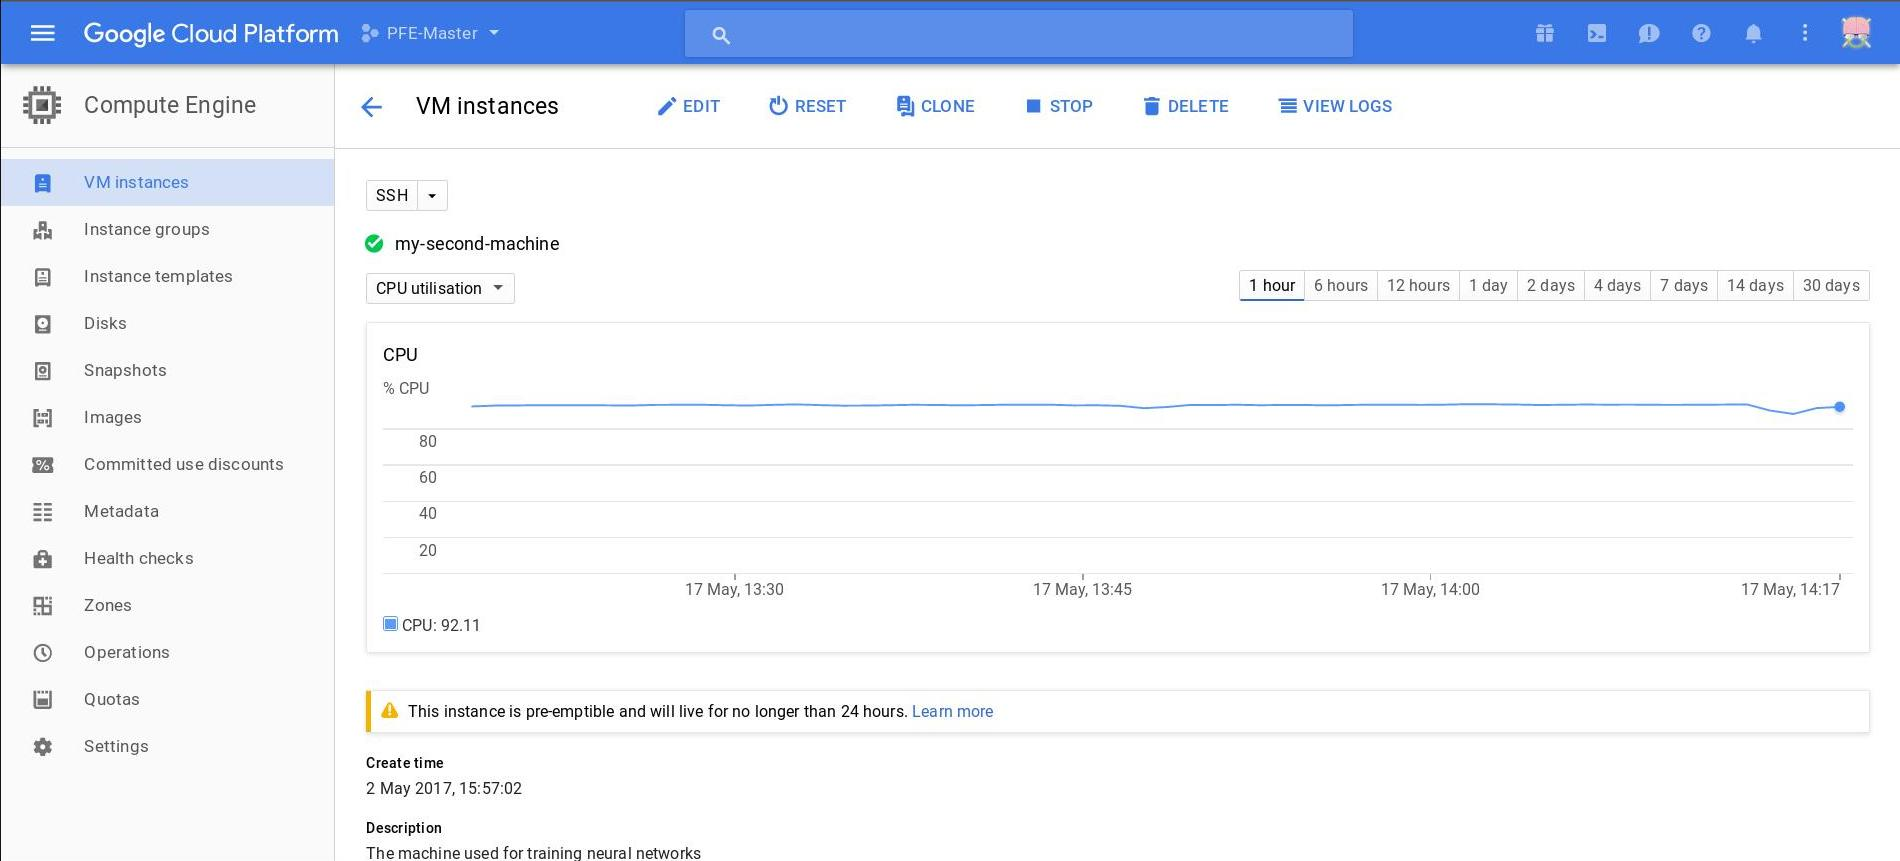
\includegraphics[width=\textwidth]{GCP-Compute}
  \caption{L'interface de gestion d'une machine virtuelle dans Compute Engine}
\end{figure}

A l'aide de ce service, nous avons créé deux machines disposant de 4 vCPU
de \keyword{Intel Xeon E5 Sandy Bridge} ayant une fréquence de base de 2.6 GHz et d'une
RAM de 15 Go. Elles ont aussi un disque dur virtuel de 10 Go où une distribution
de \keyword{GNU/Linux} est préinstallée : l'un contient \keyword{Debian 8} et l'autre
contient \keyword{CentOS 7}.

Les deux machines ont les mêmes caractéristiques, mais nous avons en effet
observé que sur la première machine (qui a \keyword{Debian 8}) le programme s'exécute
normalement mais que sur la deuxième (qui a \keyword{CentOS 7}), en raison de manque
de mémoire, il se termine sans que l'exécution soit achevée.

\subsection{Le logiciel}

Afin de réaliser un programme portable et efficace à la fois, nous avons choisi
de l'implémenter sous \keyword{Python 3}~\cite{python3} en utilisant la bibliothèque \keyword{TensorFlow}~\cite{DBLP:journals/corr/AbadiABBCCCDDDG16}
pour la création du modèle, l'apprentissage automatique et le chargement des images.
Cette bibliothèque permet d'exécuter un code de bas niveau écrit en \keyword{C++}~\cite{stroustrup1995c++}
qui peut effectuer des calculs massivement parallèles en utilisant toutes les unités
de traitement disponibles et en bénéficiant des instructions de vectorisation matérielles
existant dans ces unités. \keyword{TensorFlow} offre aussi un outil intégré
appelé \keyword{TensorBoard} permettant de dessiner le graphe du modèle et les
connexions entre ses composants, ainsi que le traçage des fonctions de performances.
Nous avons également utilisé la bibliothèque \keyword{NumPy}~\cite{walt2011numpy} pour la lecture,
le traitement et la sauvegarde des données numériques.

\begin{figure}[h]
\centering
\begin{subfigure}{0.3\textwidth}
\includegraphics[width=\textwidth]{python-logo}\end{subfigure}
\begin{subfigure}{0.3\textwidth}
\includegraphics[width=\textwidth]{TensorFlow}\end{subfigure}
\begin{subfigure}{0.3\textwidth}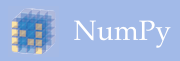
\includegraphics[width=\textwidth]{numpy_logo}\end{subfigure}
\caption{Les logos de Python, TensorFlow, et NumPy}
\end{figure}


\section{Le programme d'apprentissage}

Nous avons écrit un programme permettant d'effectuer plusieurs tâches.
D'abord, il lit la description du modèle à partir d'un fichier JSON dont
la structure est définie dans le chapitre précédent. Il est utilisé pour
construire le modèle en mémoire.

Ensuite, il fait le décodage et les transformations nécessaires des images
compressées sur le disque en mémoire et le chargement des distances et leur prétraitement.
Ce processus consomme un temps considérable et doit être évité dans les futurs lancements
du programme. Pour cela, les données traitées sont sauvegardées
sous forme brute dans le disque ce qui permet leur chargement direct.

Par la suite, l'ensemble de l'apprentissage est divisé au moment d'exécution en
sous-ensembles dits \keyword{batches} qui ont tous la même taille\footnote{
En réalité, la taille du dernier sous-ensemble n'est pas forcément égale à la
taille des autres, car cela dépend de la divisibilité de la taille de l'ensemble
sur le nombre de sous-ensembles. Par exemple, si nous avons 2454 données pour
l'apprentissage et que notre taille de batch est de 200, le dernier batch aura seulement
54 instances car 2454 n'est pas divisible par 200, ce qui nous donne un reste de 54.}.
L'ensemble de validation est chargé tel qu'il est car il est beaucoup plus petit.

L'étape suivante est le lancement de l'apprentissage. Dans le cas où il y a des
paramètres déjà enregistrés pour le modèle courant, ils sont chargés
pour continuer l'optimisation à partir du point où le programme s'est arrêté la
dernière fois. Dans l'autre cas, ils sont initialisés par des valeurs aléatoires.
L'apprentissage se fait par le passage d'un sous-ensemble d'images dans le réseau
de neurones suivi par le calcul d'erreur entre les classes de distances trouvées
par le réseau et les classes attendues. Cette erreur est minimisée à chaque
itération en appliquant la propagation arrière à l'aide de l'optimiseur.

\`A la fin de chaque itération, les nouveaux poids générés pour chaque matrice de paramètres
sont sauvegardés dans des fichiers spéciaux. Ainsi, les performances du réseau sont calculées
et enregistrées au fur et à mesure de l'avancement de ce processus pour pouvoir
suivre leur développement.

\section{Le suivi des performances}

\subsection{La technique}

Au moment de l'apprentissage, des fichiers appelés \keyword{fichiers d'événements}
contenant son avancement sont générés ou mis à jour. Ces fichiers sont persistants
et peuvent être consultés même après la terminaison du processus. Ils contiennent les graphes
représentant le changement des valeurs de l'erreur et l'exactitude en fonction
du nombre d'itérations pour chacun des deux ensembles d'apprentissage et de
validation. De plus, ils incluent une représentation graphique du modèle
d'apprentissage ayant plusieurs niveaux de détails qui affiche chaque nœud et son
rôle, ainsi que les différentes connexions entre eux et les dimensions des données
transférées. Toutes ces informations peuvent être visualisées clairement avec
l'outil \keyword{TensorBoard}.

\begin{figure}[h]
  \centering
  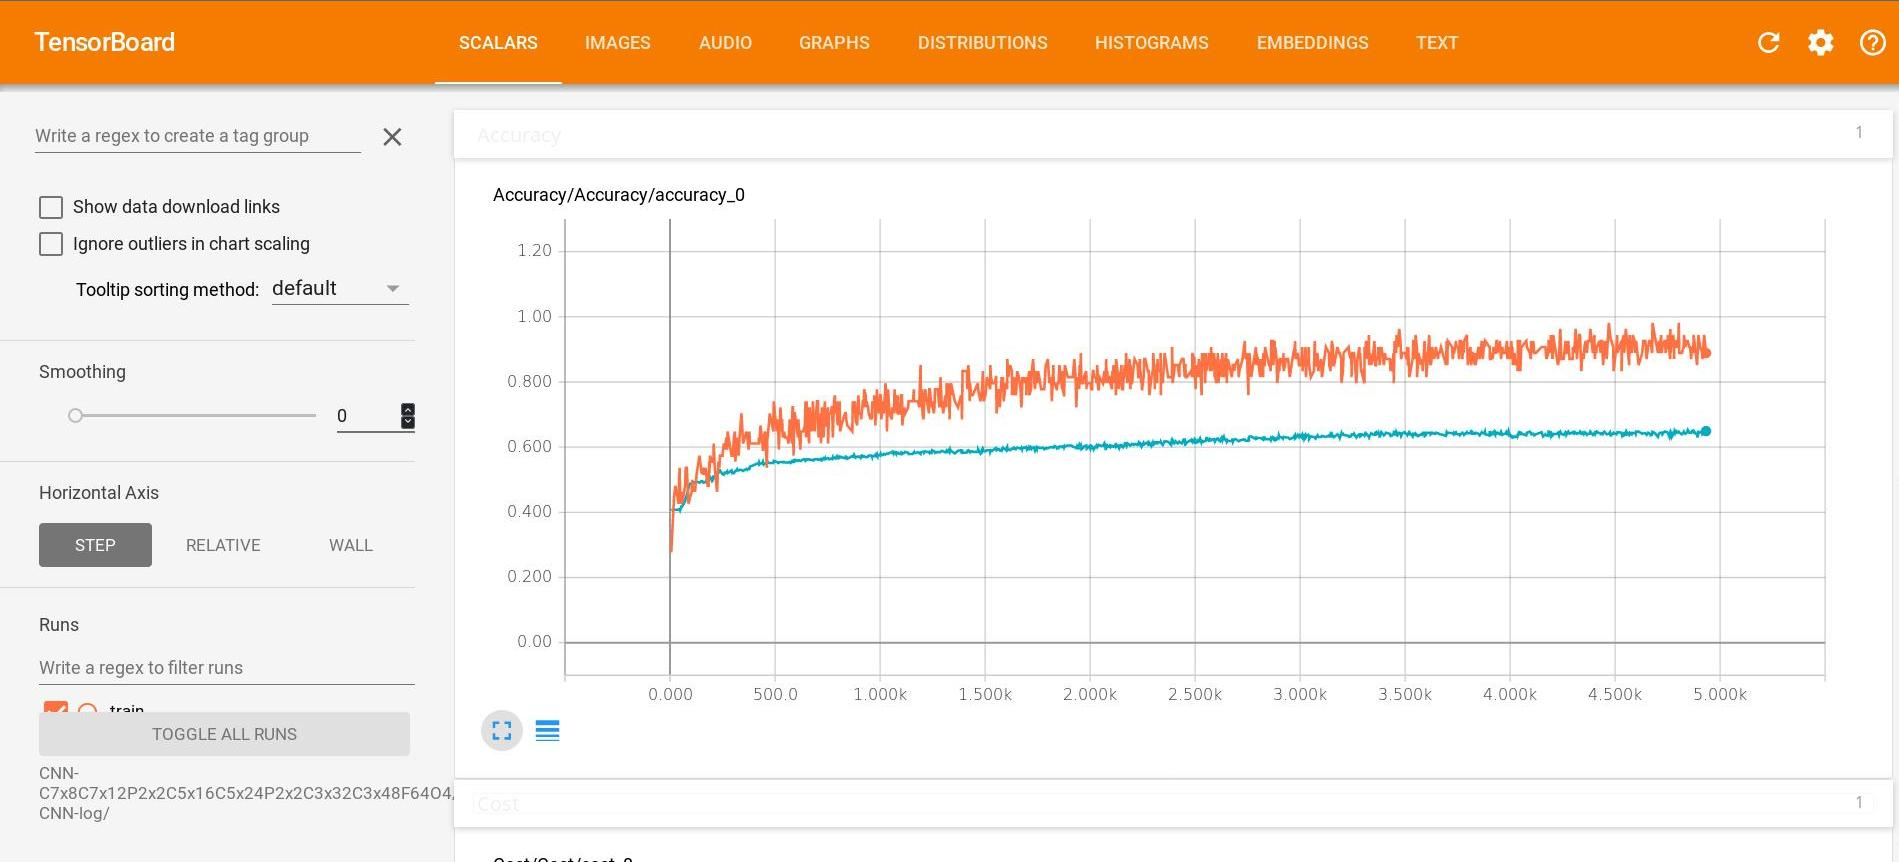
\includegraphics[width=\textwidth]{TensorBoard}
  \caption{L'interface de TensorBoard traçant les courbes de fonctions}
\end{figure}

\subsection{Les exécutions}

Nous avons effectué plusieurs exécutions en variant les configurations du modèle,
des données et de l'environnement. Chacune d'elles consomme plusieurs heures.

Nous avons commencé par l'ensemble de données du CCU. \`A base de cet ensemble,
nous avons lancé l'apprentissage de nos deux modèles. Le premier apprentissage
a été effectué sur des images de taille $48 \times 48$ (réduites par facteur de
$\frac{1}{2}$) sur le modèle le moins profond décrit dans le chapitre précédent.

Les graphes des exécutions sont présentés dans les figures suivantes. Les courbes oranges
représentent les valeurs issues de l'évaluation des performances sur le dernier batch
de données d'apprentissage et les bleues représentent celles issues de l'évaluation
sur les données de validation.

\begin{figure}[h]
\centering
\begin{subfigure}{0.8\textwidth}
  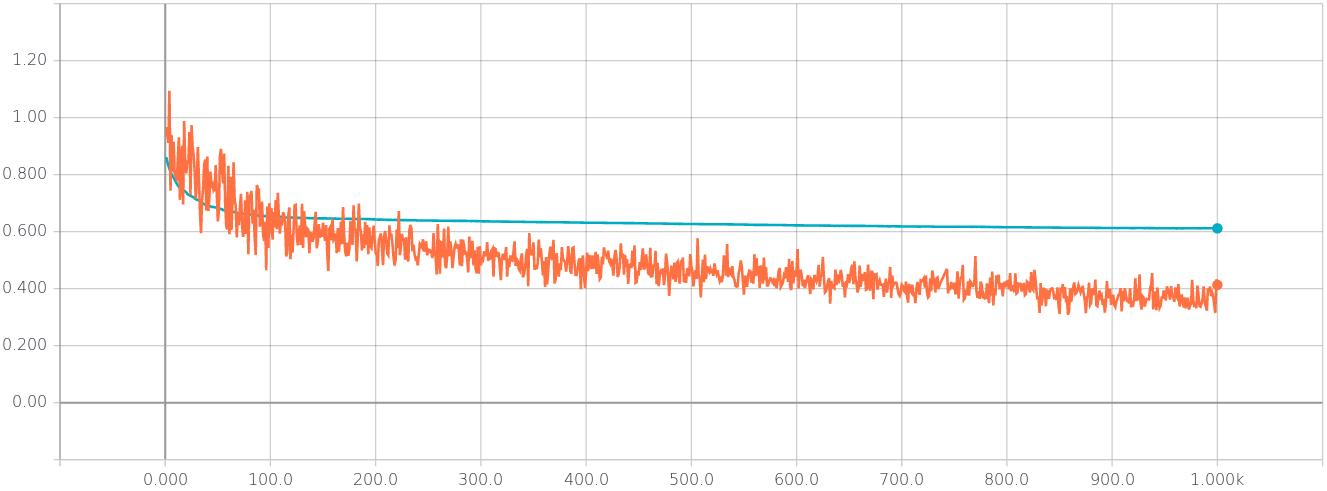
\includegraphics[width=\textwidth]{CNN-Med-CCU-Loss}
  \caption{La fonction du coût}
\end{subfigure}
\begin{subfigure}{0.8\textwidth}
  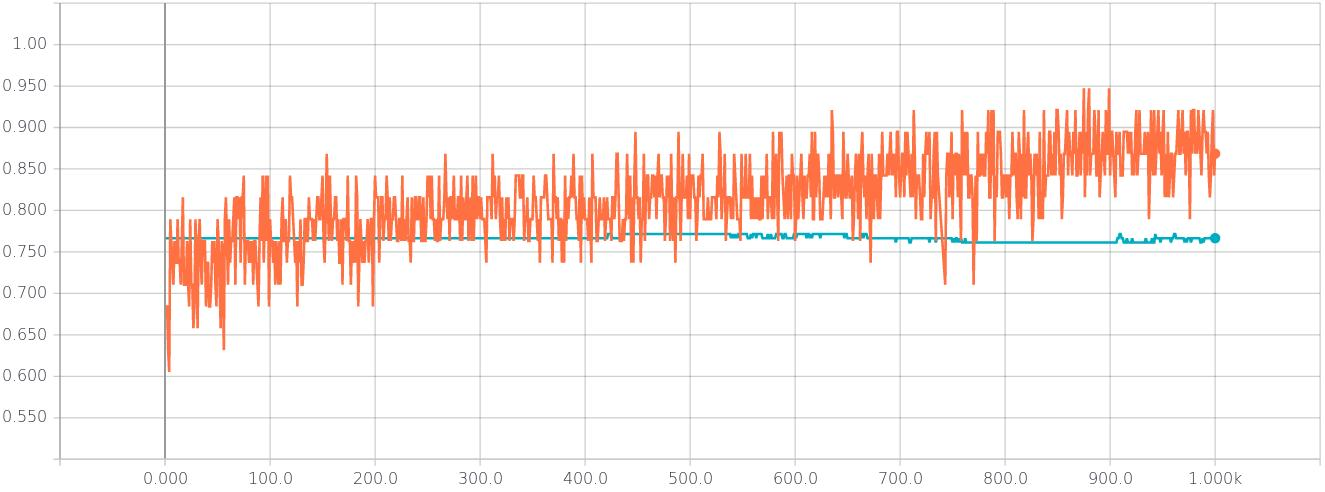
\includegraphics[width=\textwidth]{CNN-Med-CCU-Accuracy}
  \caption{La fonction d'exactitude}
\end{subfigure}
\caption{Les performances du petit réseau en utilisant l'ensemble du CCU\label{fig:med_ccu}}
\end{figure}

\`A partir du graphe de la fonction du coût, nous remarquons que les courbes
d'apprentissage et de validation divergent et que cette dernière commence
à stagner rapidement. D'autre part, l'exactitude du réseau ne s'améliore pas
pendant les $1000$ itérations, donc le réseau n'est pas capable de trouver les bons
paramètres.

Avec les mêmes données, nous avons fait une autre exécution en utilisant le grand
modèle. Les graphes de la figure \ref{fig:big_ccu} ont été obtenus.

\begin{figure}[h]
\centering
\begin{subfigure}{0.9\textwidth}
  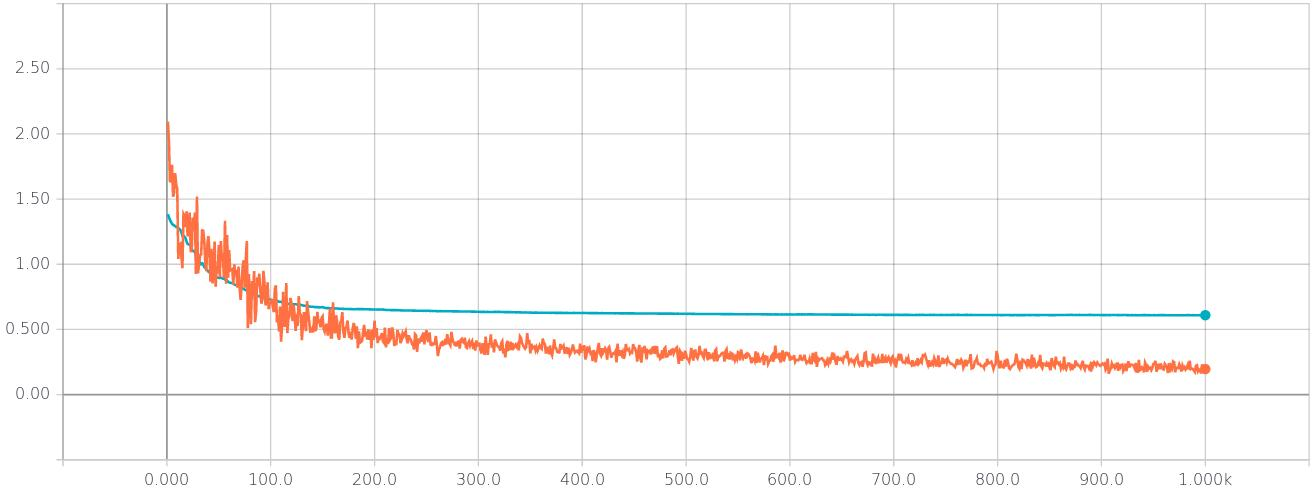
\includegraphics[width=\textwidth]{CNN-Big-CCU-Loss}
  \caption{La fonction du coût}
\end{subfigure}
\begin{subfigure}{0.9\textwidth}
  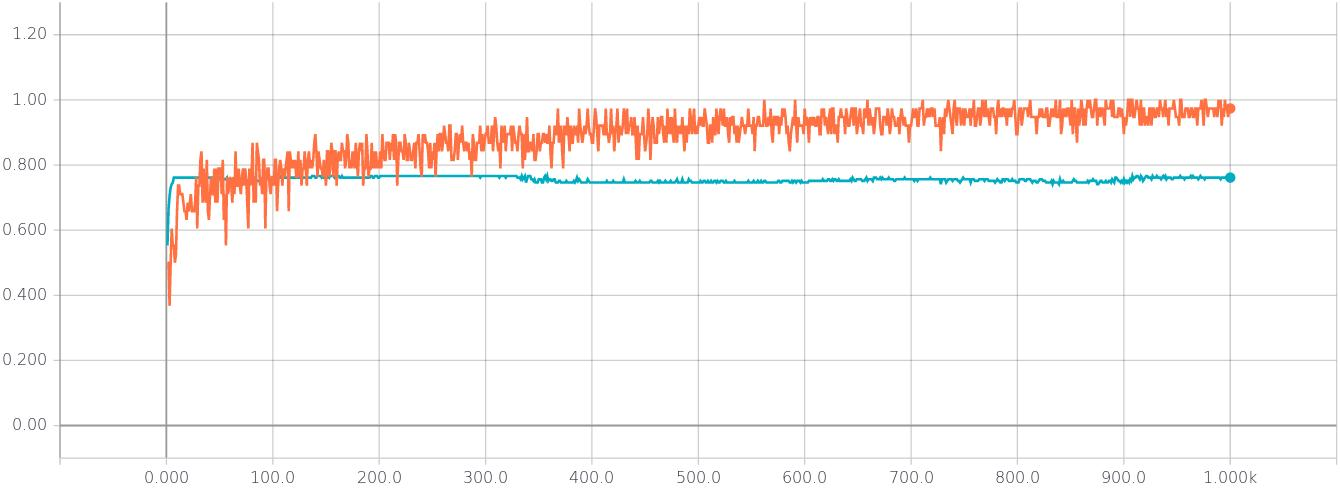
\includegraphics[width=\textwidth]{CNN-Big-CCU-Accuracy}
  \caption{La fonction d'exactitude}
\end{subfigure}
\caption{Les performances du grand réseau en utilisant l'ensemble du CCU\label{fig:big_ccu}}
\end{figure}

Nous avons recueilli les mêmes observations que celles faites pour les graphes précédents.
De plus, nous voyons que l'exactitude de validation diminue après l'itération
$330$, ce qui indique un fort sur-apprentissage.

Puisque l'augmentation de la profondeur du modèle n'a donné que de mauvais
résultats, nous pouvons conclure que le problème est causé par les données et non pas
par le modèle. Nous devons donc changer l'ensemble de données utilisé. C'est
la raison pour laquelle dans ce qui suit nous utilisons l'ensemble de données du département.

De même, nous utilisons cet ensemble pour effectuer l'apprentissage automatique
à l'aide des deux modèles utilisés précédemment. Pour chaque modèle, deux exécutions
ont été effectuées, l'une sans changer les dimensions des images (c'est à dire en
gardant leur taille originale de $96 \times 96$), et l'autre après la réduction
de la taille vers $48 \times 48$.

Les graphes de la figure \ref{fig:med_info} montrent le développement des performances
du petit modèle en utilisant des images de taille de $48 \times 48$.

\begin{figure}[h]
\centering
\begin{subfigure}{0.64\textwidth}
  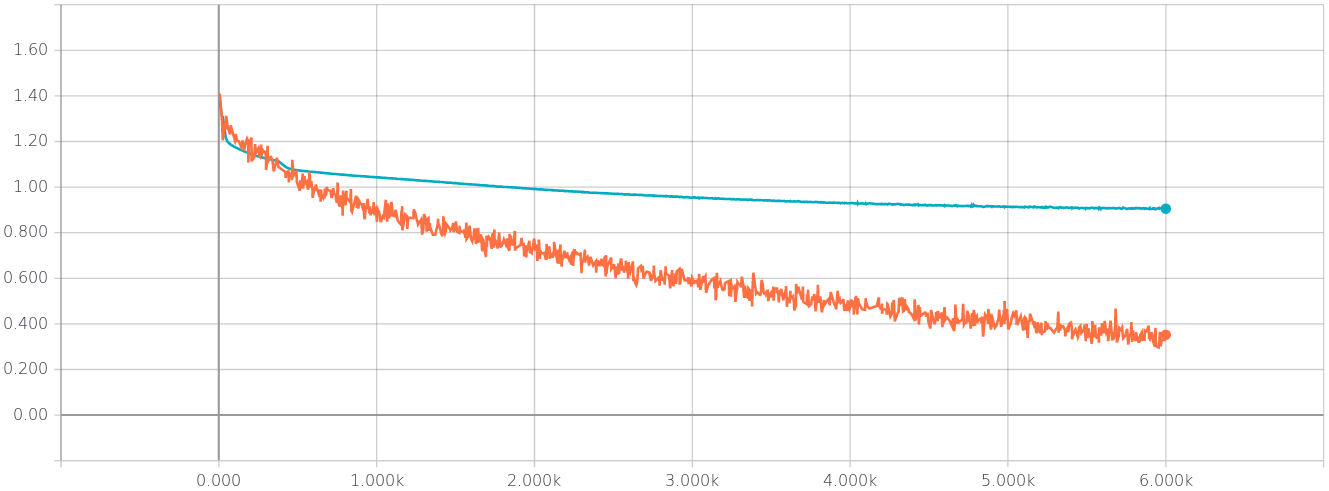
\includegraphics[width=\textwidth]{CNN-Med-Info-Loss}
  \caption{La fonction du coût}
\end{subfigure}
\begin{subfigure}{0.64\textwidth}
  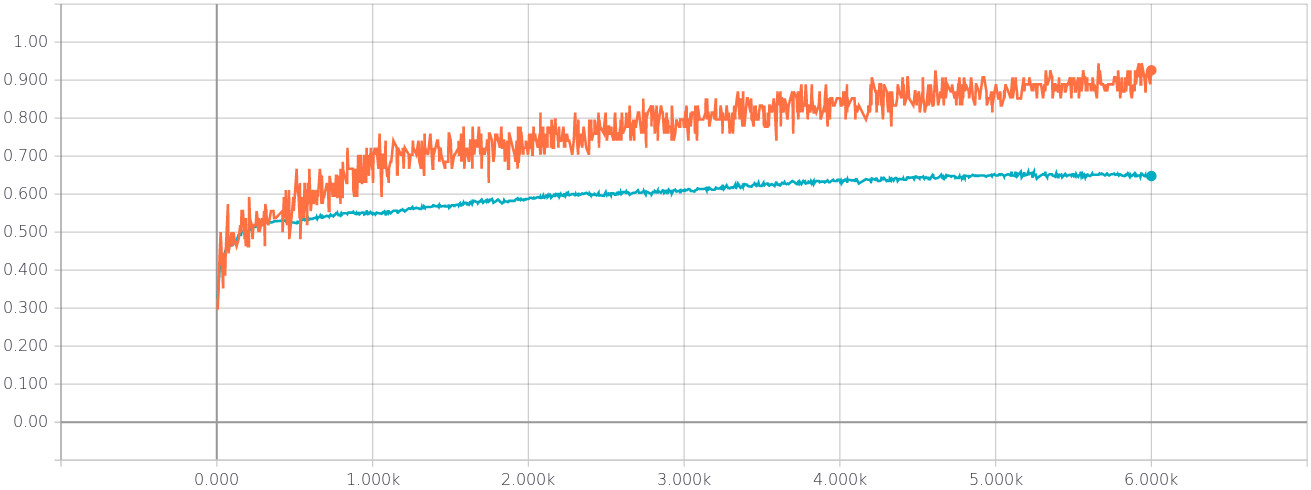
\includegraphics[width=\textwidth]{CNN-Med-Info-Accuracy}
  \caption{La fonction d'exactitude}
\end{subfigure}
\caption{Les performances du petit réseau en utilisant l'ensemble du département\label{fig:med_info}}
\end{figure}

Il est remarquable que les courbes de la fonction du coût descendent rapidement
et que celles de la fonction de l'exactitude montent normalement. La courbe de
validation de la fonction du coût stagne entre les valeurs $0.91$ et $0.9$ à partir
de l'itération $5300$. De même, la courbe de validation de la fonction d'exactitude
cesse de monter après l'itération $5000$ et continue à prendre des valeurs entre
$0.64$ et $0.65$. Cela montre que le modèle peut classifier avec un taux de
succès de $65 \%$.

En gardant la même taille d'images, nous effectuons l'apprentissage du grand modèle.
Les graphes de la figure \ref{fig:big_info} représentent le changement des performances en fonction de
nombre d'itérations.

\begin{figure}[H]
\centering
\begin{subfigure}{0.64\textwidth}
  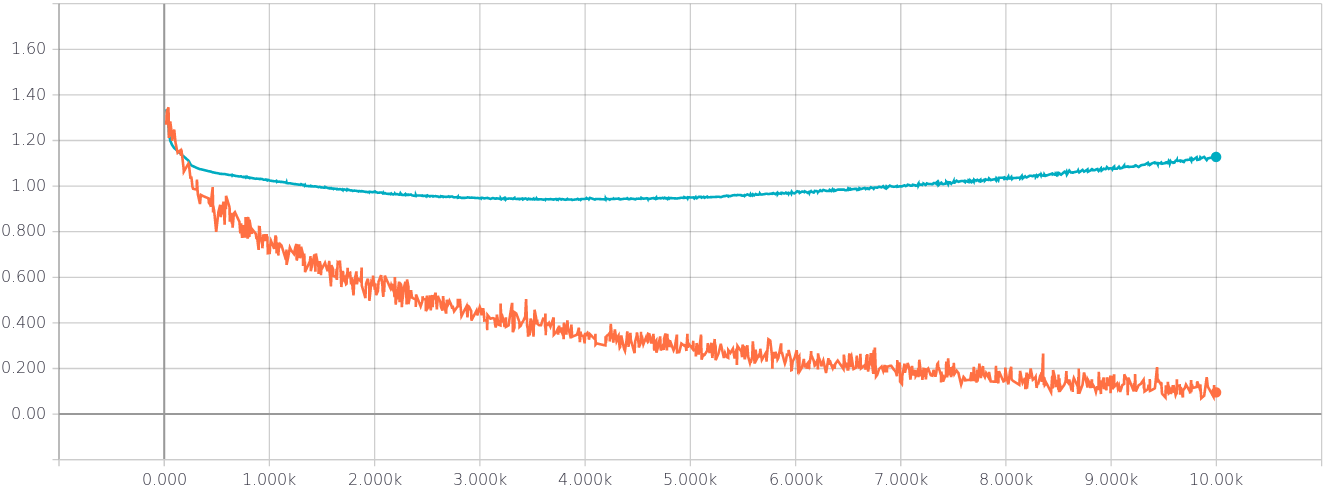
\includegraphics[width=\textwidth]{CNN-Big-Info-Loss}
  \caption{La fonction du coût}
\end{subfigure}
\begin{subfigure}{0.64\textwidth}
  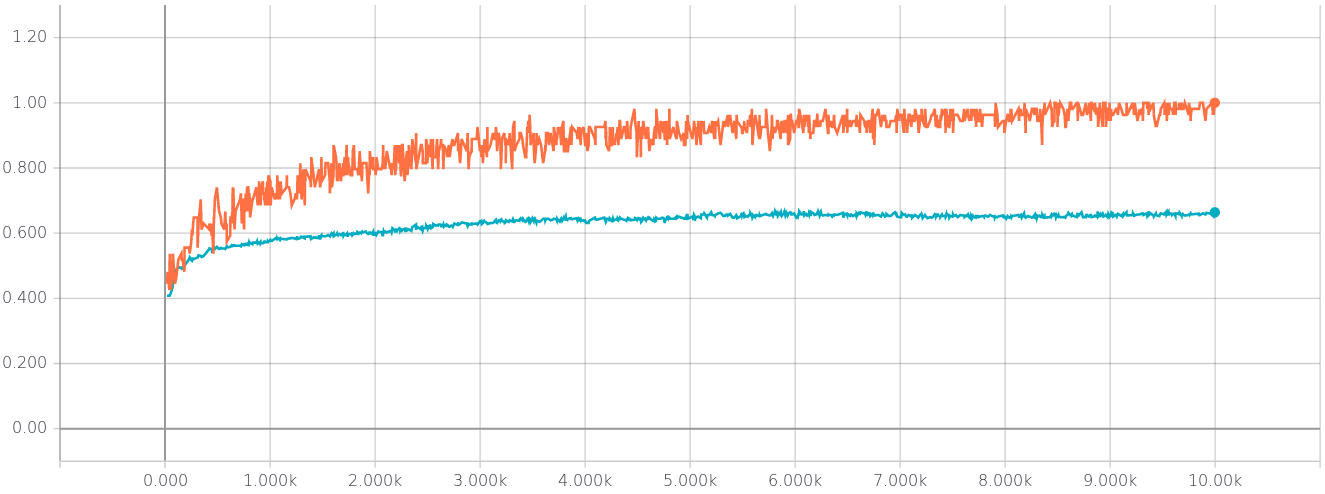
\includegraphics[width=\textwidth]{CNN-Big-Info-Accuracy}
  \caption{La fonction d'exactitude}
\end{subfigure}
\caption{Les performances du grand réseau en utilisant l'ensemble du département\label{fig:big_info}}
\end{figure}

Nous observons que les deux courbes dans les deux graphes divergent dès les
premières itérations. D'une part, l'erreur de validation augmente au lieu de diminuer
à partir de l'itération $4500$ approximativement. D'autre part, la valeur d'exactitude
commence à stagner entre $0.65$ et $0.66$ à partir de l'itération $5000$. Contrairement
aux courbes de validation, celles d'apprentissage continuent leur amélioration
à travers le temps. Ces résultats indiquent que le modèle a pu trouver la bonne
classe pour $66 \%$ des images figurant dans l'ensemble de validation.

Vu que les résultats obtenus n'étaient pas vraiment satisfaisants, nous avons essayé
d'utiliser les images sans redimensionnement, c'est à dire en gardant la taille
originale de $96 \times 96$ pixels. L'apprentissage en utilisant une telle taille
dure beaucoup plus longtemps : chaque exécution prend plusieurs jours car elle peut être
interrompue par plusieurs problèmes, comme l'arrêt imprévisible de la machine ou
une insuffisance de mémoire. C'est la raison pour laquelle nous avons évité
d'utiliser les images avec leurs taille originale au début, mais à la fin nous
sommes amenés à considérer ce choix comme une autre tentative pour améliorer les résultats.

En continuant par le même principe, nous avons utilisé les données de l'ensemble
du département pour faire l'apprentissage des deux modèles. La différence n'était
pas importante, la valeur de l'exactitude pour les deux modèles n'a pas pu
dépasser $0.67$, ce qui indique que la réduction de taille d'un facteur de $\frac{1}{2}$
pour les images de l'ensemble n'avait pas une grande influence sur les résultats obtenus.

\section{L'implémentation des modèles}

Après avoir terminé l'apprentissage de nos modèles, nous réalisons une
application qui permet à un utilisateur d'estimer la classe de distance correspondante
à l'image fournie. Cette application fonctionne sur trois éléments :

\begin{itemize}
  \item un fichier contenant la description du modèle, sous format JSON,
  \item le fichier du point de contrôle \texttt{checkpoint} qui pointe vers
  l'emplacement des fichiers qui contiennent les valeurs des paramètres du modèle,
  \item un repértoire représentant l'ensemble de test qui a le fichier \texttt{Distances.txt}
  et les images correspondantes, ou bien l'image dont il faut prédire la classe de distance.
\end{itemize}

\subsection{Chargement du réseau de neurones convolutionnel}

La première interface graphique de l'application qui s'affiche à l'ouverture est
une boîte de dialogue composée de trois parties. La première offre un champ pour
saisir l'emplacement du fichier du réseau dans le disque dur. La deuxième permet
à l'utilisateur de spécifier le chemin du fichier du point de contrôle qui permet
de charger les poids du réseau.

Dans chaque partie des deux premières, un bouton étiquetté <<Choisir>> est
disponible pour faciliter la sélection du fichier en ouvrant une boîte de
dialogue qui permet de sélectionner le fichier correspondant.
La dernière partie permet de spécifier les paramètres d'images utilisées lors de
l'apprentissage du modèle. Ces paramètres représentent les trois dimensions de l'image
(la hauteur, la largeur et le nombre de canaux).

\begin{figure}[h]
  \centering
  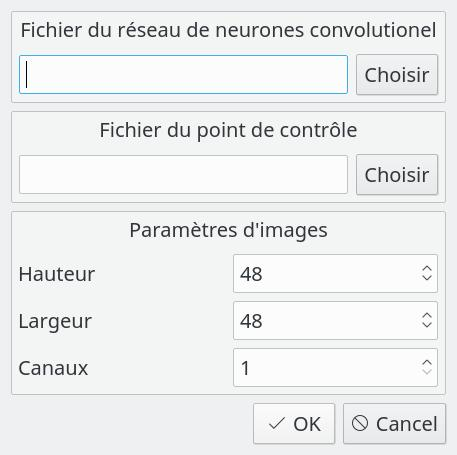
\includegraphics[width=0.4\textwidth]{cnn_loader}
  \caption{La boîte de dialogue de sélection des fichiers de configuration}
\end{figure}

\begin{figure}[h]
\centering
\begin{subfigure}{0.49\textwidth}
  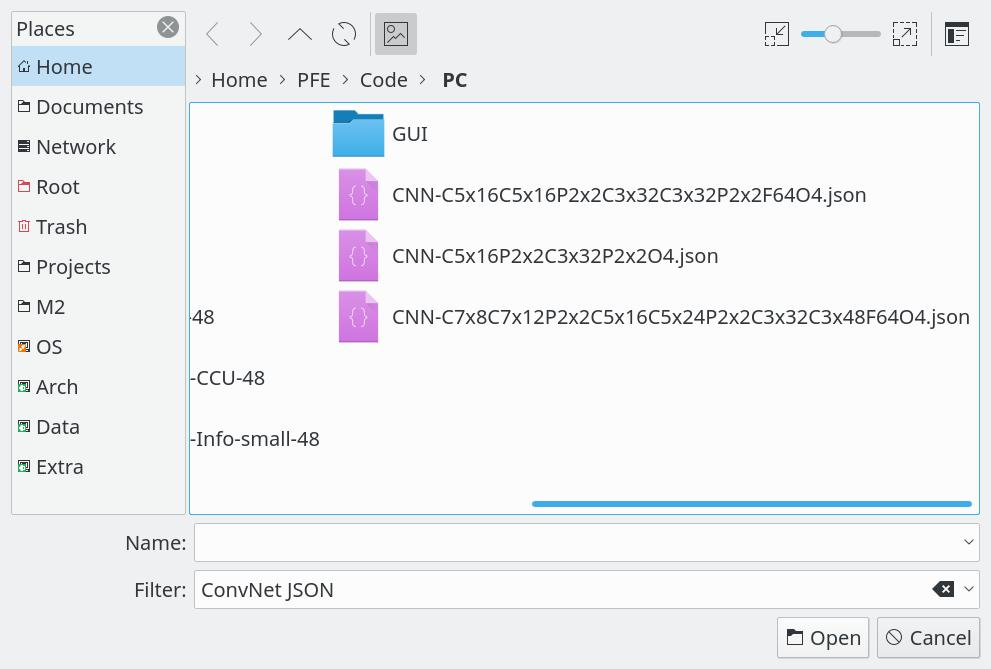
\includegraphics[width=\textwidth]{open_ConvNet}
  \caption{Sélection du fichier du réseau}
\end{subfigure}
\begin{subfigure}{0.49\textwidth}
  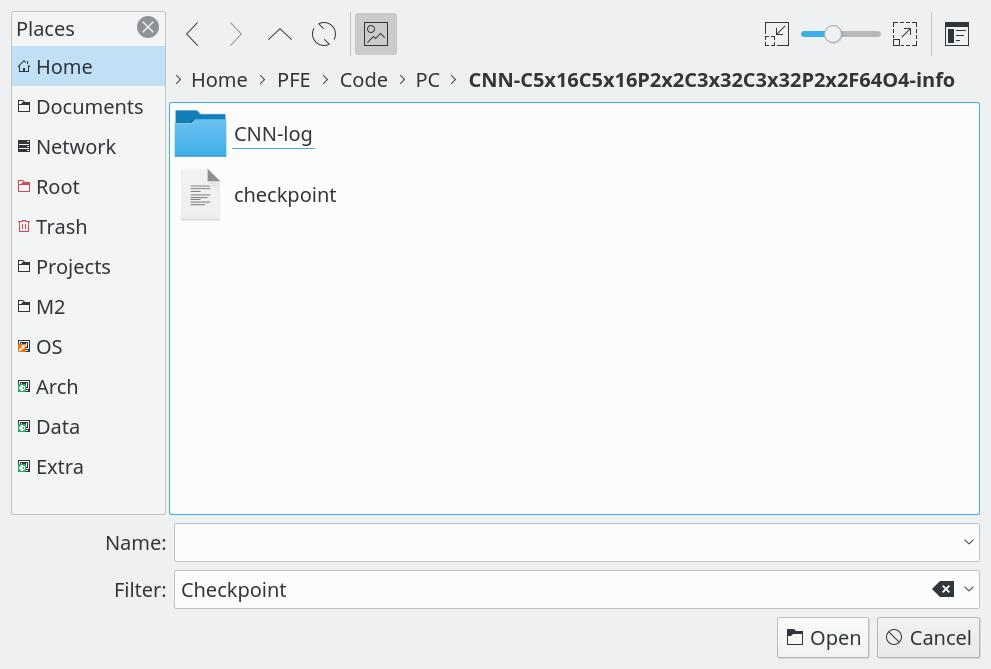
\includegraphics[width=\textwidth]{open_checkpoint}
  \caption{Sélection du fichier de point de contrôle}
\end{subfigure}
\caption{Les boîtes de dialogue de sélection des fichiers}
\end{figure}

\subsection{Test et prédiction}

Après avoir donné toutes ces informations, l'interface précédente est cachée
pour qu'une autre s'ouvre. La nouvelle interface graphique contient deux sous-interfaces
dont une est visible à la fois. L'une d'elles est celle du test et l'autre est
celle de la prédiction. Toutes les deux contiennent un champ où l'utilisateur
doit introduire le chemin de ses données.

\begin{figure}[h]
\centering
\begin{subfigure}{0.4\textwidth}
  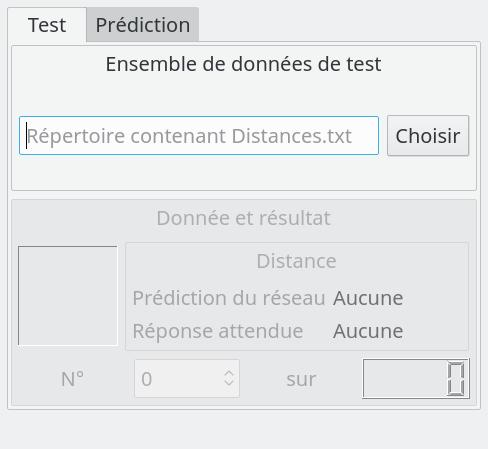
\includegraphics[width=\textwidth]{test_tab}
  \caption{La sous-interface du test}
\end{subfigure}
\begin{subfigure}{0.4\textwidth}
  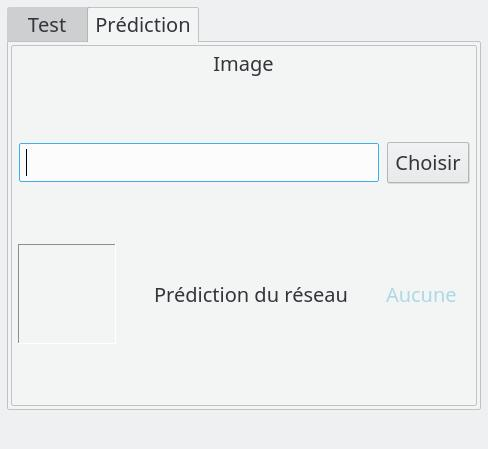
\includegraphics[width=\textwidth]{predict_tab}
  \caption{La sous-interface de la prédiction}
\end{subfigure}
\caption{Les sous-interfaces}
\end{figure}

\subsubsection{Le test}

En utilisant l'interface du test, l'utilisateur peut spécifier le chemin d'un
répertoire contenant son ensemble de données. Ce répertoire doit contenir le fichier
\texttt{Distances.txt} qui doit être enregistré sous la structure décrite dans
\ref{subsec:format}, et aussi toutes les images correspondant
aux lignes de ce fichier, dont chacune a un nom respectant le format indiqué dans \ref{subsec:format}.

L'utilisateur peut saisir le chemin manuellement dans le champ ou à l'aide du bouton
<<Choisir>>. Dès que le chemin devient valide, l'ensemble de données est chargé
et la première instance est sélectionnée automatiquement. L'utilisateur peut
changer l'instance en modifiant le nombre affiché. Pour chaque instance, la classe
prédite par le réseau est affichée en bleu et la classe réelle en vert. La première
est trouvée par le passage de l'image à travers le réseau et la lecture du résultat,
et la deuxième est récuperée à partir du fichier des distances.

\parbox[][1em][]{\textwidth}{}

\begin{figure}[h]
\centering
\begin{subfigure}{0.32\textwidth}
  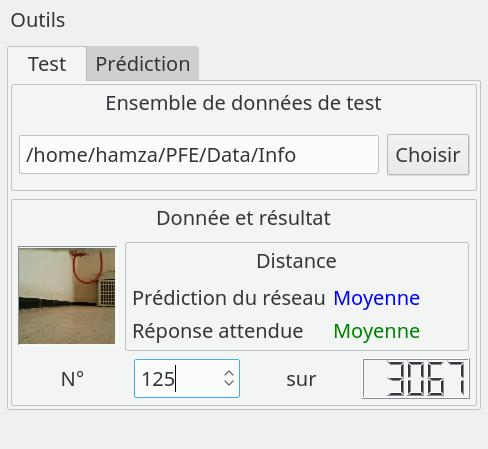
\includegraphics[width=\textwidth]{test_tab_1}
\end{subfigure}
\begin{subfigure}{0.32\textwidth}
  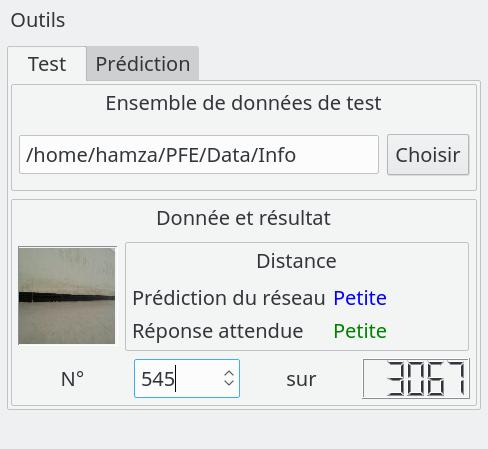
\includegraphics[width=\textwidth]{test_tab_2}
\end{subfigure}
\begin{subfigure}{0.32\textwidth}
  \includegraphics[width=\textwidth]{test_tab_3}
\end{subfigure}
\caption{L'interface du test}
\end{figure}

\subsubsection{La prédiction}

Contrairement à la première interface, la deuxième permet à l'utilisateur de
spécifier le chemin d'une seule image ayant les mêmes propriétés que les images
de test et dont la classe est inconnue. \`A cause de cela, seule la réponse
du réseau est disponible. Nous ne pouvons donc pas comparer son résultat avec
une référence. En effet, cette fonctionnalité représente le but de ce projet.

Le fonctionnement de l'interface est pratiquement le même que celui de la première.
Quand l'utilisateur saisit un chemin valide d'une image manuellement ou en utilisant
le bouton <<Choisir>>, l'image est affichée et elle est passée au réseau pour
déterminer sa classe de distances. Cette réponse est affichée sur l'interface.

\begin{figure}[h]
\centering
\begin{subfigure}{0.32\textwidth}
  \includegraphics[width=\textwidth]{predict_tab_1}
\end{subfigure}
\begin{subfigure}{0.32\textwidth}
  \includegraphics[width=\textwidth]{predict_tab_2}
\end{subfigure}
\begin{subfigure}{0.32\textwidth}
  \includegraphics[width=\textwidth]{predict_tab_3}
\end{subfigure}
\caption{L'interface de la prédiction}
\end{figure}

\section{Le test des modèles}

En utilisant notre application et des ensembles de données de test, nous pouvons
réaliser l'évaluation de nos modèles. Nous prenons donc quelques instances de
l'ensemble de validation du département qui sont des instances non vues par le
réseau lors de l'apprentissage.

L'ensemble de validation que nous avons créé contient $613$ instances. Vu la grandeur
de ce nombre, nous ne pouvons pas présenter ici les résultats issues de toutes les
images de l'ensemble. Nous nous limitons donc à quelques instances dont le réseau
a pu trouver la bonne réponse et quelques autres dont il n'a pas trouvé la bonne réponse.

\subsection{Le modèle le moins profond}

Nous avons effectué les tests en utilisant des images de taille réduite ($48 \times 48$)
et celles de taille originale ($96 \times 96$). La première colonne contient
l'image utilisée, la seconde représente la classe prédite par le réseau, et la dernière
représente la classe réelle. Les résultats sont disponibles dans les tableaux suivants.

\begin{table}[H]
  \centering
  \begin{tabular}{|m{0.095\textwidth} m{0.1\textwidth} m{0.12\textwidth}|m{0.095\textwidth} m{0.1\textwidth} m{0.12\textwidth}|}
    \hline
    Image & Prédiction & Correction & Image & Prédiction & Correction \\
    \hline
    \includegraphics[width=0.09\textwidth]{test_info_2} & Petite & Petite & \includegraphics[width=0.09\textwidth]{test_info_4} & Petite & Petite \\
    \includegraphics[width=0.09\textwidth]{test_info_6} & Petite & Grande & \includegraphics[width=0.09\textwidth]{test_info_8} & Moyenne & Moyenne \\
    \includegraphics[width=0.09\textwidth]{test_info_10} & Moyenne & Moyenne & \includegraphics[width=0.09\textwidth]{test_info_12} & Petite & Inconnue \\
    \includegraphics[width=0.09\textwidth]{test_info_14} & Petite & Petite & \includegraphics[width=0.09\textwidth]{test_info_16} & Moyenne & Moyenne \\
    \includegraphics[width=0.09\textwidth]{test_info_18} & Moyenne & Moyenne & \includegraphics[width=0.09\textwidth]{test_info_20} & Petite & Petite \\
    \hline
  \end{tabular}
  \caption{Résultats des tests sur le petit modèle en utilisant les images réduites}
\end{table}

\begin{table}[H]
  \centering
  \begin{tabular}{|m{0.095\textwidth} m{0.1\textwidth} m{0.12\textwidth}|m{0.095\textwidth} m{0.1\textwidth} m{0.12\textwidth}|}
    \hline
    Image & Prédiction & Correction & Image & Prédiction & Correction \\
    \hline
    \includegraphics[width=0.09\textwidth]{test_info_2} & Petite & Petite & \includegraphics[width=0.09\textwidth]{test_info_4} & Petite & Petite \\
    \includegraphics[width=0.09\textwidth]{test_info_6} & Grande & Grande & \includegraphics[width=0.09\textwidth]{test_info_8} & Moyenne & Moyenne \\
    \includegraphics[width=0.09\textwidth]{test_info_10} & Moyenne & Moyenne & \includegraphics[width=0.09\textwidth]{test_info_12} & Inconnue & Inconnue \\
    \includegraphics[width=0.09\textwidth]{test_info_14} & Inconnue & Petite & \includegraphics[width=0.09\textwidth]{test_info_16} & Moyenne & Moyenne \\
    \includegraphics[width=0.09\textwidth]{test_info_18} & Moyenne & Moyenne & \includegraphics[width=0.09\textwidth]{test_info_20} & Petite & Petite \\
    \hline
  \end{tabular}
  \caption{Résultats des tests sur le petit modèle en utilisant les images originales}
\end{table}

\subsection{Le modèle le plus profond}

De plus, nous avons réalisé les mêmes expérimentations avec le grand modèle. Les
résultats que nous avons obtenus sont présentés dans les tableaux suivants.

\begin{table}[H]
  \centering
  \begin{tabular}{|m{0.095\textwidth} m{0.1\textwidth} m{0.12\textwidth}|m{0.095\textwidth} m{0.1\textwidth} m{0.12\textwidth}|}
    \hline
    Image & Prédiction & Correction & Image & Prédiction & Correction \\
    \hline
    \includegraphics[width=0.09\textwidth]{test_info_2} & Petite & Petite & \includegraphics[width=0.09\textwidth]{test_info_4} & Petite & Petite \\
    \includegraphics[width=0.09\textwidth]{test_info_6} & Grande & Grande & \includegraphics[width=0.09\textwidth]{test_info_8} & Moyenne & Moyenne \\
    \includegraphics[width=0.09\textwidth]{test_info_10} & Moyenne & Moyenne & \includegraphics[width=0.09\textwidth]{test_info_12} & Inconnue & Inconnue \\
    \includegraphics[width=0.09\textwidth]{test_info_14} & Petite & Petite & \includegraphics[width=0.09\textwidth]{test_info_16} & Moyenne & Moyenne \\
    \includegraphics[width=0.09\textwidth]{test_info_18} & Moyenne & Moyenne & \includegraphics[width=0.09\textwidth]{test_info_20} & Petite & Petite \\
    \hline
  \end{tabular}
  \caption{Résultats des tests sur le grand modèle en utilisant les images réduites}
\end{table}

\begin{table}[H]
  \centering
  \begin{tabular}{|m{0.095\textwidth} m{0.1\textwidth} m{0.12\textwidth}|m{0.095\textwidth} m{0.1\textwidth} m{0.12\textwidth}|}
    \hline
    Image & Prédiction & Correction & Image & Prédiction & Correction \\
    \hline
    \includegraphics[width=0.09\textwidth]{test_info_2} & Petite & Petite & \includegraphics[width=0.09\textwidth]{test_info_4} & Petite & Petite \\
    \includegraphics[width=0.09\textwidth]{test_info_6} & Petite & Grande & \includegraphics[width=0.09\textwidth]{test_info_8} & Moyenne & Moyenne \\
    \includegraphics[width=0.09\textwidth]{test_info_10} & Moyenne & Moyenne & \includegraphics[width=0.09\textwidth]{test_info_12} & Petite & Inconnue \\
    \includegraphics[width=0.09\textwidth]{test_info_14} & Inconnue & Petite & \includegraphics[width=0.09\textwidth]{test_info_16} & Moyenne & Moyenne \\
    \includegraphics[width=0.09\textwidth]{test_info_18} & Moyenne & Moyenne & \includegraphics[width=0.09\textwidth]{test_info_20} & Petite & Petite \\
    \hline
  \end{tabular}
  \caption{Résultats des tests sur le grand modèle en utilisant les images originales}
\end{table}

\section{Conclusion}

Dans ce chapitre, nous avons présenté les différentes approches que nous avons suivies
afin d'effectuer l'apprentissage de nos réseaux de neurones convolutionnels. Ces
approches consistent à varier les données et leurs dimensions, ainsi que les modèles
utilisés. Nous avons également présenté la majorité des graphes de performances
et les résultats obtenus après avoir fait la simulation avec des données de test,
ainsi que l'application utilisée pour les réaliser.

Avec un taux d'exactitude maximal égal à $67 \%$ approximativement, nous pouvons
conclure que les résultats obtenus n'étaient pas très bons, et que cela est causé par
plusieurs facteurs. D'une part, les données sont hétérogènes, car les images contiennent
des objets de nature et de forme très différente. D'autre part, les capteurs
ultrasoniques utilisés ne sont pas fiables et peuvent retourner de mauvaises valeurs
dans certaines conditions, sans mentionner leur limite de mesure pour les objets
distants. De plus, les ensembles de données que nous avons construits sont biaisés
et nous n'avons pas le nombre nécessaire de données pour les équilibrer.
